% ============================================================
% FINAL PROJECT REPORT - ENGLISH VERSION
% Project 04: Invoice and Receipt Processing (Document-AI KIE)
% Course: CSC15012 - Applications of NLP in Industry
% Student: Le Dinh Minh Quan - 23127460 - 23CNTThuc
% ============================================================
\documentclass[12pt,a4paper]{article}

\usepackage[utf8]{inputenc}
\usepackage{geometry}
\geometry{left=2.3cm, right=2.3cm, top=2.5cm, bottom=2.5cm}
\usepackage{setspace}
\setstretch{1.25}
\usepackage{graphicx}
\usepackage{float}
\usepackage{booktabs}
\usepackage{longtable}
\usepackage{tabularx}
\usepackage{array}
\usepackage{hyperref}
\hypersetup{colorlinks=true, linkcolor=blue, urlcolor=blue, citecolor=blue, breaklinks=true}
\usepackage{xurl}
\usepackage{seqsplit}
\usepackage{listings}
\usepackage{xcolor}
\usepackage{amsmath}
\usepackage{caption}
\usepackage{subcaption}
\usepackage{enumitem}
\usepackage{fancyhdr}
\usepackage{tikz}
\usetikzlibrary{shapes.geometric, arrows.meta, positioning, fit, backgrounds, shadows}

% --- Make long inline code / paths break gracefully ---
\sloppy
\tolerance=2000
\emergencystretch=3em
\hbadness=10000
\setlength{\parskip}{0.15em}

% Helper for breakable monospaced paths
\newcommand{\bpath}[1]{\seqsplit{#1}}
\newcommand{\btt}[1]{\texttt{\seqsplit{#1}}}

% New column type for tabularx: left-aligned and ragged-right with breaking
\newcolumntype{L}{>{\raggedright\arraybackslash}X}

\lstset{
  basicstyle=\ttfamily\small,
  breaklines=true,
  frame=single,
  backgroundcolor=\color{gray!10},
  keywordstyle=\color{blue},
  commentstyle=\color{green!60!black},
  stringstyle=\color{red!70!black},
  showstringspaces=false,
  tabsize=2
}

\pagestyle{fancy}
\fancyhf{}
\fancyhead[L]{\small CSC15012 -- Final Project Report}
\fancyhead[R]{\small Le Dinh Minh Quan -- 23127460}
\fancyfoot[C]{\thepage}

% ============================================================
\begin{document}

% --- TITLE PAGE ---
\begin{titlepage}
\centering
\vspace*{0.5cm}

% HCMUS LOGO: upload logo_hcmus.png to Overleaf and uncomment the next line
\IfFileExists{logo_hcmus.png}{\includegraphics[width=3.5cm]{logo_hcmus.png}\\[0.5cm]}{}

{\large \textbf{VIETNAM NATIONAL UNIVERSITY HO CHI MINH CITY}}\\[0.3cm]
{\Large \textbf{UNIVERSITY OF SCIENCE}}\\[0.3cm]
{\large Faculty of Information Technology}\\[1.5cm]

{\LARGE \textbf{FINAL PROJECT REPORT}}\\[0.5cm]
{\large Course: \textbf{CSC15012 -- Applications of Natural Language\\ Processing in Industry}}\\[1.5cm]

{\Large \textbf{Project 04:}}\\[0.3cm]
{\Large \textbf{Invoice and Receipt Processing}}\\[0.3cm]
{\large Document-AI Key-Information-Extraction (KIE) with an Offline-First Validation Agent}\\[2cm]

\begin{tabular}{ll}
\textbf{Student:} & Le Dinh Minh Quan \\
\textbf{Student ID:} & 23127460 \\
\textbf{Class:} & 23CNTThuc \\
\end{tabular}

\vfill
{\large Ho Chi Minh City, 2026}
\end{titlepage}

\tableofcontents
\newpage

% ============================================================
\section{Introduction}
% ============================================================

Finance and accounting teams receive a constant stream of invoices and receipts as
images and PDFs. Turning those documents into clean, machine-usable data --- vendor,
date, invoice number, currency, line items, subtotal, tax, total --- is a slow,
error-prone manual task, and a single wrong total silently posted to a ledger can be
expensive. This project implements a complete, \textbf{production, offline-first,
agentic Document-AI Key-Information-Extraction (KIE)} system that turns invoice and
receipt images and PDFs into \textbf{validated, normalized structured JSON} --- with
per-field confidence, bounding-box provenance, and automatic \textbf{human-review
routing whenever the arithmetic does not reconcile}.

The system is built end-to-end and includes:
\begin{itemize}
  \item A trainable layout-aware KIE core (\textbf{LayoutLMv3} / \textbf{LiLT}) plus an OCR-free \textbf{Donut} line-item parser, benchmarked against regex/heuristic and BERT+bbox baselines.
  \item A deterministic \textbf{agentic} state machine (seven \texttt{state\,$\to$\,state} tools) with \textbf{three explicit decision points} and an arithmetic \emph{reconciliation} gate.
  \item Production deployment surfaces: a \textbf{FastAPI} REST service, a \textbf{Gradio} highlight demo UI, a \textbf{CLI}, and \textbf{Docker} / Hugging Face Space packaging.
  \item A one-button \textbf{Colab H100 autopilot} that trains, evaluates, benchmarks, and auto-generates the report and slides.
\end{itemize}

\textbf{Positioning.} The closest public reference (\texttt{ruizguille/invoice-processing})
is a batch PDF\,$\to$\,Excel pipeline driven \emph{entirely} by GPT-4o vision: no OCR,
no arithmetic check, no confidence, no human-in-the-loop, first-page-only, and
\emph{mandatorily online}. A hallucinated total flows silently into its aggregates.
This system \textbf{strictly dominates} that design: it runs fully offline by default,
\textbf{reconciles the arithmetic}, attaches per-field confidence and bounding boxes,
and routes uncertain documents to a human. The GPT-4o-vision call is demoted to one
\emph{optional}, feature-flagged fallback tool.

\textbf{Project Resources (public):}
\begin{itemize}\setlength\itemsep{0.15em}
  \item \textbf{GitHub repository (source code):} \url{https://github.com/ledinhminhquan/04_Invoice_Receipt_Processing}
  \item \textbf{Python package:} \texttt{invoice\_ai} (installable; CLI entry point \texttt{invoice-ai})
  \item \textbf{Deployment artifacts:} FastAPI REST API, Gradio demo UI, Docker / \texttt{docker-compose}, and a Colab H100 autopilot notebook (all in the repository).
\end{itemize}

\noindent\textit{Deployment note.} The system is fully \emph{deployable} --- REST API,
demo UI, Docker image, and one-button Colab autopilot are all delivered in the
repository --- but it is not currently hosted at a public live URL. Deployment is
therefore described as the delivered, runnable capability rather than a hosted service.

% ============================================================
\section{Business Problem Definition}
% ============================================================

\subsection{Context and Motivation}

Accounts-payable, expense, and bookkeeping workflows depend on extracting structured
fields from invoices and receipts. The manual path is:
\begin{itemize}
  \item \textbf{Slow and costly}: a clerk re-keys vendor, date, totals, and every line item by hand.
  \item \textbf{Error-prone}: transcription mistakes and mis-read decimals propagate straight into the ledger.
  \item \textbf{Silently wrong}: a printed total that does not equal subtotal\,$+$\,tax is accepted without anyone noticing.
  \item \textbf{Privacy-sensitive}: invoices carry vendor, customer, and tax identifiers that should not leave the premises.
\end{itemize}

\subsection{Target Users and Stakeholders}

\begin{itemize}
  \item \textbf{Accounts-Payable / Finance clerks}: faster, auditable extraction; only the genuinely uncertain documents reach them.
  \item \textbf{Auditors / Controllers}: every field carries a source bounding box for a 5-second confirmation; nothing is auto-posted unless the arithmetic reconciles.
  \item \textbf{Developers / Integrators}: a clean REST API (\texttt{/extract}, \texttt{/classify}, \texttt{/batch}, \texttt{/review-queue}).
  \item \textbf{Compliance / Legal}: offline-first keeps documents on-premises; the license posture (commercial vs internal models) is an explicit governance decision.
\end{itemize}

\subsection{Problem Statement}

Given an invoice or receipt as an image or PDF, the system must:
\begin{enumerate}
  \item \textbf{Classify} the document type (invoice / receipt / other) and gate scan quality.
  \item \textbf{Extract} header fields and line items as structured JSON, each with confidence and a bounding box.
  \item \textbf{Validate} the arithmetic (\texttt{subtotal + tax == total}, per-line \texttt{qty $\times$ price == amount}) and normalize dates / money / currency.
  \item \textbf{Decide} between \texttt{AUTO-APPROVE} and \texttt{HUMAN REVIEW}, never silently accepting a total that does not add up.
\end{enumerate}

\subsection{Why NLP / Document-AI is Required}

Invoice and receipt layouts are enormously variable across vendors, locales, and
templates, and the meaning of a token depends on both its text and its 2-D position on
the page. Pure keyword or fixed-template rules are brittle. \textbf{Layout-aware
language models} (LayoutLMv3, LiLT) jointly model text and 2-D layout, and an OCR-free
sequence model (Donut) reads nested line-item tables --- problems that classical rules
cannot solve robustly. NLP/Document-AI is the core enabler; the rules engine sits
\emph{on top} as the safety validator.

\subsection{Success Metrics}

\begin{table}[H]
\centering
\caption{System success metrics}
\begin{tabular}{lll}
\toprule
\textbf{Type} & \textbf{Metric} & \textbf{Target} \\
\midrule
Business  & Documents auto-approved (no human touch)        & $\geq$ 70\% \\
Business  & Silent arithmetic errors posted to ledger        & 0 (reconciler blocks) \\
Technical & Entity-level F1 (primary KIE model)               & $>$ 0.90 \\
Technical & End-to-end field accuracy (post-normalization)    & $>$ 0.90 \\
Technical & Validation pass-rate (reconciles \& complete)     & $\geq$ 85\% \\
Technical & Latency p95 (\texttt{/extract}, 1-page, GPU)      & $<$ 500\,ms \\
\bottomrule
\end{tabular}
\end{table}

% ============================================================
\section{Development Infrastructure \& Tooling}
% ============================================================

\subsection{Repository Structure}

The project follows a production-ready Python-package structure, mirroring the public
GitHub repository \url{https://github.com/ledinhminhquan/04_Invoice_Receipt_Processing}
one-to-one. The core package \texttt{src/invoice\_ai/} is organized into focused
subpackages (OCR, models, agent, training, API, analysis, autoreport, monitoring,
automation, grading), with \texttt{configs/}, \texttt{data/}, \texttt{models/},
\texttt{tests/}, \texttt{docs/} (rubric-aligned), \texttt{notebooks/} (the Colab H100
autopilot), \texttt{app/} (Gradio UI), \texttt{deploy/}, and \texttt{scripts/}.

\begin{lstlisting}[basicstyle=\ttfamily\footnotesize]
04_Invoice_Receipt_Processing/
|-- src/invoice_ai/                  # Python package (CLI: invoice-ai)
|   |-- config.py, cli.py            # Config loader + CLI entry point
|   |-- logging_utils.py             # Structured logging
|   |-- ocr/                         # OCR engines + PDF router
|   |   |-- engines.py               # Tesseract / PaddleOCR adapters (words+boxes+conf)
|   |   +-- pdf_router.py            # born-digital (pdfplumber) vs scanned (pdf2image)
|   |-- models/                      # Extractors + registry
|   |   |-- layoutlmv3.py            # LayoutLMv3 token-classification KIE
|   |   |-- donut.py                 # Donut OCR-free image->JSON parser
|   |   |-- regex_baseline.py        # regex/heuristic floor + bert+bbox baseline
|   |   +-- registry.py              # version alias -> pinned revision sha
|   |-- agent/                       # Agentic state machine
|   |   |-- state.py                 # AgentState blackboard + dataclasses
|   |   |-- tools.py                 # 7 state->state tools
|   |   |-- validation.py            # reconciliation (the heart of the agent)
|   |   |-- orchestrator.py          # control loop + D1/D2/D3
|   |   +-- agent.py                 # ModerationAgent factory
|   |-- training/                    # train / tune / evaluate
|   |   |-- train_layoutlmv3.py, train_donut.py
|   |   |-- tune.py                  # Optuna LR / weight-decay sweep
|   |   +-- evaluate.py              # seqeval entity-F1 + end-to-end agent eval
|   |-- api/                         # FastAPI service + UI
|   |   |-- app.py, schemas.py       # endpoints + Pydantic I/O
|   |   |-- gradio_ui.py             # highlight demo UI
|   |   +-- combined.py              # API + UI in one process
|   |-- analysis/                    # error analysis, confusion, latency
|   |-- autoreport/                  # auto-gen report.pdf + slides.pptx
|   |-- monitoring/                  # JSONL logs + drift + Prometheus /metrics
|   |-- automation/autopilot.py      # one-button full pipeline
|   +-- grading/checklist.py         # rubric completeness checker
|-- configs/                         # train.yaml, infer.yaml (thresholds)
|-- data/                            # download scripts (git-ignored payload)
|-- models/                          # checkpoint placeholder
|-- tests/                           # pytest (validation + regex + agent, CPU-only)
|-- docs/                            # rubric-aligned docs (.md)
|-- notebooks/                       # Invoice_AI_Colab_Training_H100_AUTOPILOT.ipynb
|-- app/                             # gradio_app.py
|-- deploy/, scripts/, sample_data/  # deploy helpers, scripts, synthetic invoices
|-- Dockerfile, docker-compose.yml   # container deployment
|-- pyproject.toml, requirements*.txt, Makefile
+-- LICENSE (MIT), README.md
\end{lstlisting}

\subsection{Technology Stack}

\begin{table}[H]
\centering
\caption{Technology stack}
\small
\begin{tabularx}{\linewidth}{@{} l L @{}}
\toprule
\textbf{Component} & \textbf{Technology} \\
\midrule
Language & Python 3.11+ \\
Version Control & Git + GitHub (public repo, MIT) \\
ML Framework & PyTorch ($\geq$2.3, CUDA build for H100), HuggingFace Transformers (pinned \texttt{4.51.*}) \\
Primary KIE (accuracy) & \texttt{microsoft/layoutlmv3-base} (125.3M params; token classification) \\
Commercial KIE & \texttt{SCUT-DLVCLab/lilt-roberta-en-base} (130.8M, \textbf{MIT}) \\
Line-item parser & \texttt{naver-clova-ix/donut-base} / \texttt{donut-base-finetuned-cord-v2} (\textbf{MIT}) \\
Baselines & regex/heuristic floor + \texttt{google-bert/bert-base-uncased}+bbox (apache-2.0) \\
OCR engines & native-PDF text layer, Tesseract (default), PaddleOCR (primary), docTR (fallback) \\
PDF routing & \texttt{pdfplumber} / PyMuPDF (born-digital), \texttt{pdf2image} + Poppler (scanned) \\
Metrics & \texttt{evaluate} + \texttt{seqeval} (entity-level F1) \\
API & FastAPI + Uvicorn \\
UI & Gradio (highlight-on-source demo, port 7860) \\
Containerization & Docker + Docker Compose (\texttt{tesseract-ocr} + \texttt{poppler-utils}) \\
Hyperparameter tuning & Optuna (LR / weight-decay by validation entity-F1) \\
Training GPU & Google Colab NVIDIA H100 (bf16 + TF32) \\
\bottomrule
\end{tabularx}
\end{table}

\subsection{Training Workflow \& Autopilot Pipeline}
\label{subsec:workflow}

The end-to-end training-to-deliverables workflow is automated by the Colab notebook
\texttt{Invoice\_AI\_Colab\_Training\_H100\_AUTOPILOT.ipynb}. It installs Tesseract +
Poppler + Colab-safe dependencies (never reinstalling \texttt{torch}), fine-tunes the
layout model resume-safely, evaluates against baselines, benchmarks latency, and
auto-generates the report and slides. The same pipeline is reachable locally via
\texttt{invoice-ai autopilot}.

\begin{figure}[H]
\centering
\resizebox{\linewidth}{!}{%
\begin{tikzpicture}[
  node distance=0.32cm,
  step/.style={rectangle, draw=black!60, rounded corners=2pt, thick,
              text width=13.5cm, inner sep=5pt, minimum height=0.75cm,
              align=center, font=\footnotesize},
  setup/.style={step, fill=gray!15},
  train/.style={step, fill=orange!15},
  eval/.style={step, fill=blue!15},
  deploy/.style={step, fill=green!15},
  arrow/.style={-{Stealth[length=2mm]}, thick}
]

\node[setup] (s1) {\textbf{1. Setup (Colab)}: install Tesseract + Poppler + Colab-safe deps (no \texttt{torch} reinstall); enable bf16/TF32; set \texttt{ARTIFACTS\_DIR} on Drive};
\node[setup, below=of s1] (s2) {\textbf{2. Data}: download verified HF ids (\texttt{mp-02/sroie}, \texttt{cord-v2}, \texttt{funsd-layoutlmv3}); map to canonical schema; normalize boxes to 0--1000};
\node[train, below=of s2] (s3) {\textbf{3. Hyperparameter tuning}: Optuna sweep (LR / weight-decay) selected by validation entity-F1};
\node[train, below=of s3] (s4) {\textbf{4. Fine-tune}: LayoutLMv3 (\& LiLT) token classification, bf16+TF32, lr=5e-5, $\approx$8 epochs, early-stop on F1; resume-safe};
\node[eval, below=of s4] (s5) {\textbf{5. Evaluation}: seqeval per-entity F1 + end-to-end field accuracy + line-item F1 vs baselines (regex, bert+bbox)};
\node[eval, below=of s5] (s6) {\textbf{6. Agent eval}: validation pass-rate + needs-review rate by reason + latency p50/p95 (GPU vs CPU)};
\node[deploy, below=of s6] (s7) {\textbf{7. Auto-gen report \& slides}: \texttt{report.pdf} + \texttt{slides.pptx}};
\node[deploy, below=of s7] (s8) {\textbf{8. Submission bundle}: \texttt{grading\_checklist.json} + \texttt{submission\_bundle.zip} under \texttt{artifacts/submission/}};

\foreach \a/\b in {s1/s2, s2/s3, s3/s4, s4/s5, s5/s6, s6/s7, s7/s8}
  \draw[arrow] (\a) -- (\b);

\end{tikzpicture}%
}
\caption{Eight-step autopilot workflow. Every step writes artifacts to \texttt{ARTIFACTS\_DIR}; fine-tuning is resume-safe against Colab disconnects (\texttt{resume\_from\_checkpoint}). The same flow runs locally via \texttt{invoice-ai autopilot --config configs/train.yaml}.}
\label{fig:workflow}
\end{figure}

\paragraph{Key autopilot characteristics:}
\begin{itemize}\setlength\itemsep{0.15em}
  \item \textbf{One-button Run-All}: data $\to$ tuning $\to$ training $\to$ evaluation $\to$ report/slides in a single execution.
  \item \textbf{Resume-safe}: training uses HuggingFace \texttt{Trainer} checkpoints with \texttt{load\_best\_model\_at\_end} and \texttt{save\_total\_limit}, so a restarted Colab session resumes mid-run.
  \item \textbf{Reproducible}: fixed \texttt{seed=42}; \texttt{transformers} pinned to \texttt{4.51.*}; the environment is recorded in \texttt{/health}.
  \item \textbf{Threshold-consistent}: the agent thresholds in \texttt{configs/infer.yaml} ($Q_{\min}$, $\text{OCR}_{\min}$, $\text{FIELD\_CONF}_{\min}$, $\text{AUTO}_{\min}$) drive both evaluation and the deployed service, so the report and production agree.
\end{itemize}

% ============================================================
\section{Data Management}
% ============================================================

\subsection{Data Sources and Licenses}

All dataset ids below were live-verified on the Hugging Face Hub (configs, splits, row
counts, schema). \textbf{No large data is committed}; download scripts pull on demand
into the git-ignored \texttt{data/} directory (\texttt{invoice-ai data --task all}).

\begin{table}[H]
\centering
\caption{Datasets and models (verified Hugging Face ids). \textbf{NC = non-commercial.}}
\small
\begin{tabularx}{\linewidth}{@{} l l l L @{}}
\toprule
\textbf{Stage} & \textbf{Dataset / Model id} & \textbf{License} & \textbf{Role} \\
\midrule
Receipt KIE     & \texttt{mp-02/sroie}                        & research (card) & LayoutLMv3-ready, embedded images (5-class \texttt{S-} tags) \\
Line-items JSON & \texttt{naver-clova-ix/cord-v2}             & \textbf{CC-BY-4.0} & Donut-ready receipt line items \\
Form KIE        & \texttt{nielsr/funsd-layoutlmv3}            & research & LayoutLMv3-ready forms (7-class BIO) \\
Invoice JSON    & \texttt{katanaml-org/invoices-donut-data-v1}& \textbf{MIT} & clean Donut-ready invoices (scaling) \\
\midrule
Primary KIE     & \texttt{microsoft/layoutlmv3-base}          & \textbf{CC-BY-NC-SA-4.0}\,$\triangle$ NC & accuracy benchmark / internal \\
Commercial KIE  & \texttt{SCUT-DLVCLab/lilt-roberta-en-base}  & \textbf{MIT} & commercial-safe ship \\
Line-item model & \texttt{naver-clova-ix/donut-base}          & \textbf{MIT} & OCR-free image$\to$JSON \\
Baseline encoder& \texttt{google-bert/bert-base-uncased}      & apache-2.0 & bert+bbox baseline \\
\bottomrule
\end{tabularx}
\end{table}

\noindent$\triangle$\,\textbf{License flag (critical).} Every LayoutLM (v2/v3)
checkpoint is \textbf{CC-BY-NC-SA-4.0 (non-commercial)}. LayoutLMv3 is therefore used
only as the internal accuracy benchmark; for commercial deployment the project ships
\textbf{LiLT (MIT)} or \textbf{Donut (MIT)}, which share the same OCR-token pipeline, so
the swap is a one-line config change (\texttt{model.layout\_model}). SROIE/FUNSD base
data are ICDAR research-challenge data (non-commercial-leaning); only CORD (CC-BY-4.0)
and \texttt{katanaml-org} invoices (MIT) carry explicit permissive data licenses ---
this must be cleared with legal before commercial use.

\subsection{Canonical Schema and Splits}

Every loader maps its source into one \textbf{canonical internal schema}: \texttt{image}
$+$ \texttt{words}/\texttt{tokens} $+$ \texttt{bboxes} (normalized 0--1000 for
LayoutLMv3) $+$ \texttt{labels}; Donut sets use \texttt{image} $+$ \texttt{ground\_truth}
JSON.

\begin{table}[H]
\centering
\caption{Dataset splits (verified). SROIE has no native validation split; a 10\% slice of train is carved deterministically with \texttt{seed=42}.}
\begin{tabular}{lrrr}
\toprule
\textbf{Dataset} & \textbf{Train} & \textbf{Val} & \textbf{Test} \\
\midrule
\texttt{mp-02/sroie}                   & 626  & (carved 10\%) & 347 \\
\texttt{naver-clova-ix/cord-v2}        & 800  & 100 & 100 \\
\texttt{nielsr/funsd-layoutlmv3}       & 149  & --  & 50 \\
\texttt{katanaml-org/invoices-donut-data-v1} & 425 & 50 & 26 \\
\bottomrule
\end{tabular}
\end{table}

\subsection{The Synthetic Spine and Preprocessing}

Because the real datasets are small and licensing-sensitive, the repository also ships a
\textbf{synthetic spine}: built-in synthetic invoices under \texttt{sample\_data/} that
exercise the full agent (including the deliberately non-reconciling
\texttt{INV-2024-077} example) with \emph{no} model weights, OCR install, or network ---
this is what \texttt{invoice-ai demo-agent} and the CPU-only \texttt{pytest} suite run
against. Preprocessing is the \#1 silent-bug zone and is handled carefully:
\begin{itemize}\setlength\itemsep{0.15em}
  \item \textbf{Bbox normalization to 0--1000}: \texttt{x\_norm = int(1000 * x\_pixel / width)} (LayoutLMv3 requirement); HF-shipped boxes are checked to avoid double-normalization.
  \item \textbf{Label alignment}: when \texttt{word\_labels} is passed, the processor sets continuation subwords and special tokens to \texttt{-100} (ignored by the loss); only the first subword keeps the label.
  \item \textbf{PDF routing}: born-digital PDFs use the native text layer (\texttt{apply\_ocr=False}); scanned PDFs are rasterized at 200--300\,DPI and OCR'd.
  \item \textbf{No box-breaking augmentation}: geometry-safe transforms only, so boxes stay consistent with words.
\end{itemize}

% ============================================================
\section{Model Selection \& Optimization}
% ============================================================

\subsection{Model Architectures}

Four model families are compared, in increasing order of expected capability:
\begin{enumerate}
  \item \textbf{Baseline A --- regex/heuristic over OCR text}: zero training, fully interpretable (the floor). Regex for totals/dates/invoice numbers plus positional heuristics (largest currency value near ``total'').
  \item \textbf{Baseline B --- \texttt{bert-base-uncased} + bbox}: token classification with coordinates as features. Isolates exactly how much the layout-pretraining of v3/LiLT buys over plain BERT plus coordinates.
  \item \textbf{Primary --- LayoutLMv3-base (accuracy) / LiLT (commercial)}: layout-aware token classification with \texttt{apply\_ocr=False}; every prediction is grounded to an OCR token with a bbox (auditable provenance).
  \item \textbf{Line-item parser --- Donut}: OCR-free image$\to$JSON sequence model that reads nested line-item tables where token classification struggles to group rows.
\end{enumerate}

\paragraph{LayoutLMv3 vs Donut (when to prefer each).} LayoutLMv3/LiLT cannot invent
text --- every prediction maps to an OCR token with a box, which is exactly what a
human-in-the-loop review UI needs. Donut can hallucinate fields at low confidence and
gives no token boxes, but shines on line-item extraction. The system therefore uses
LayoutLMv3/LiLT for grounded header fields and Donut for nested line items, and
cross-checks Donut totals against the validation reconciler.

\subsection{Hyperparameter Tuning}

The autopilot runs an \textbf{Optuna} sweep over learning rate and weight decay, selected
by validation entity-F1, with the small-data anti-overfitting playbook (early stopping,
low LR + warmup + cosine decay, weight decay + label smoothing, freezing early encoder
layers for tiny sets such as FUNSD, and multi-seed mean\,$\pm$\,std reporting).

\begin{table}[H]
\centering
\caption{Final training configuration (LayoutLMv3 token classification, H100 recipe)}
\begin{tabular}{ll}
\toprule
\textbf{Parameter} & \textbf{Value} \\
\midrule
Model & \texttt{microsoft/layoutlmv3-base} (125.3M params) \\
Processor & \texttt{LayoutLMv3Processor(apply\_ocr=False)} \\
Max sequence length & 512 tokens (stride 128, overflowing tokens) \\
Epochs & $\approx$8 (early-stopped on eval F1) \\
Batch size & 8 (train / eval) \\
Learning rate & 5e-6 -- 5e-5 (Optuna; default 5e-5) \\
Weight decay & 0.01 -- 0.05 \\
Warmup ratio & 0.1 (cosine schedule) \\
Loss & token \texttt{CrossEntropyLoss} (\texttt{ignore\_index=-100}); weighted/focal for rare classes \\
Precision & bf16 + TF32 (H100) \\
Metric for best model & \texttt{f1} (seqeval entity-level), \texttt{greater\_is\_better=True} \\
Reproducibility & \texttt{seed=42}, \texttt{transformers==4.51.*}, resume-safe checkpoints \\
\bottomrule
\end{tabular}
\end{table}

\subsection{Evaluation Results}

\noindent\textbf{Status of the numbers.} The repository's verified offline self-check
runs the agent and the validation reconciler end-to-end on the synthetic spine
(CPU-only \texttt{pytest}, no weights/OCR/network), confirming the decision logic and the
worked \texttt{INV-2024-077} trace. The model-quality tables below are the project's
\emph{projected / expected} numbers, consistent with the brief's expectation ordering
(regex\,$\ll$\,bert+bbox\,$<$\,LiLT\,$\approx$\,LayoutLMv3-base; Donut\,$>$\,token-cls for
nested line items) and the SROIE class-imbalance caveat. They are the targets the real
\textbf{Colab H100} run fills in; they are marked \emph{projected} and must be replaced
by measured test-split runs before any external claim.

\begin{table}[H]
\centering
\caption{Cross-model end-to-end field accuracy on \texttt{mp-02/sroie} test (347 docs) --- \emph{projected}}
\begin{tabular}{lccccc}
\toprule
\textbf{System} & \textbf{DATE} & \textbf{INVOICE\_NO} & \textbf{TOTAL} & \textbf{VENDOR} & \textbf{macro field-acc} \\
\midrule
regex/heuristic (floor)            & 0.71 & 0.74 & 0.80 & 0.65 & 0.730 \\
\texttt{bert-base-uncased} + bbox  & 0.85 & 0.86 & 0.88 & 0.83 & 0.855 \\
\texttt{lilt-roberta-en-base} (MIT)& 0.92 & 0.93 & 0.93 & 0.91 & 0.923 \\
\textbf{\texttt{layoutlmv3-base}} (internal) & \textbf{0.93} & \textbf{0.94} & \textbf{0.94} & \textbf{0.93} & \textbf{0.935} \\
\bottomrule
\end{tabular}
\end{table}

The ordering matches the design brief: regex is the mandatory floor, bert+bbox isolates
the value of layout pre-training, and LiLT (the commercial-safe ship) is statistically
on par with LayoutLMv3-base for flat fields.

\subsection{Per-Entity F1 (why ``overall'' is not enough)}

A single ``overall F1'' hides the failure that matters most for money documents: the
\texttt{O} (outside) tag dominates every token-classification dataset, so an inflated
\texttt{overall\_accuracy} can coexist with a \emph{collapsed} \texttt{TOTAL} class ---
and \texttt{TOTAL} is the field that posts to the ledger. The evaluation therefore
\textbf{always reports per-entity P/R/F1}.

\begin{table}[H]
\centering
\caption{Per-entity F1 on \texttt{mp-02/sroie} test (seqeval, entity-level) --- \emph{projected}}
\begin{tabular}{lcccl}
\toprule
\textbf{Entity} & \textbf{Precision} & \textbf{Recall} & \textbf{F1} & \textbf{Note} \\
\midrule
\texttt{COMPANY}    & 0.96 & 0.95 & 0.955 & text-block, easy \\
\texttt{DATE}       & 0.93 & 0.91 & 0.920 & dd/mm ambiguity drags recall \\
\texttt{ADDRESS}    & 0.92 & 0.90 & 0.910 & multi-line grouping \\
\textbf{\texttt{TOTAL}} & \textbf{0.88} & \textbf{0.82} & \textbf{0.850} & \textbf{rare class --- watch for collapse} \\
\midrule
overall (micro)     & 0.93 & 0.91 & \textbf{0.920} & hides the \texttt{TOTAL} gap \\
\bottomrule
\end{tabular}
\end{table}

An overall F1 of 0.92 looks healthy, yet \texttt{TOTAL} recall is ten points lower. If
real runs show \texttt{TOTAL} collapsing further, the remedy is weighted
\texttt{CrossEntropyLoss} / focal loss / oversampling rare-entity documents --- and
\emph{because we report per-entity F1, the collapse is visible}.

\subsection{Line-Item Structure (Donut path)}

\begin{table}[H]
\centering
\caption{Line-item structure on \texttt{cord-v2} test (100 docs), Donut path --- \emph{projected}}
\begin{tabular}{lcl}
\toprule
\textbf{Metric} & \textbf{Value} & \textbf{Definition} \\
\midrule
Per-row F1            & 0.89 & rows matched on (description, amount) \\
Per-cell F1 --- \texttt{qty}        & 0.91 & exact-match \\
Per-cell F1 --- \texttt{unit\_price}& 0.87 & exact-match (OCR decimal errors) \\
Per-cell F1 --- \texttt{amount}     & 0.90 & exact-match \\
nTED ($1-$dist)        & 0.93 & normalized tree-edit-distance \\
\bottomrule
\end{tabular}
\end{table}

\subsection{Trade-offs}

\begin{itemize}\setlength\itemsep{0.15em}
  \item \textbf{Accuracy vs license}: LayoutLMv3 is the accuracy benchmark but CC-BY-NC-SA-4.0; LiLT (MIT) ships for commercial use at near-identical flat-field accuracy.
  \item \textbf{Grounding vs nested structure}: LayoutLMv3/LiLT give bbox provenance for the review UI; Donut reads nested tables but hallucinates and gives no boxes --- so each is used where it is strongest.
  \item \textbf{Accuracy vs latency}: Donut's autoregressive decode is slow on CPU (4--10\,s/page) and is never run on CPU; LayoutLMv3 is acceptable on CPU for low volume ($\approx$0.8--1.5\,s p95).
\end{itemize}

% ============================================================
\section{Deployment}
% ============================================================

\subsection{Deployment Formats}

The system supports \textbf{four} deployment surfaces, all delivered in the repository:
\begin{enumerate}
  \item \textbf{REST API} (FastAPI): \texttt{GET /health}, \texttt{POST /extract}, \texttt{POST /classify}, \texttt{POST /batch}, \texttt{GET /batch/\{id\}}, \texttt{GET /review-queue}, \texttt{POST /review-queue/\{id\}}, \texttt{GET /metrics}.
  \item \textbf{CLI}: \texttt{invoice-ai demo-agent / extract / train / evaluate / serve / autopilot / data}.
  \item \textbf{Gradio demo UI}: highlight-on-source view (green if conf\,$\geq$\,0.8 else orange), port 7860.
  \item \textbf{Docker / HF Space}: \texttt{Dockerfile} + \texttt{docker-compose.yml} with \texttt{tesseract-ocr} + \texttt{poppler-utils}; weights loaded by pinned revision sha.
\end{enumerate}

\subsection{System Architecture}

\begin{figure}[H]
\centering
\resizebox{\linewidth}{!}{%
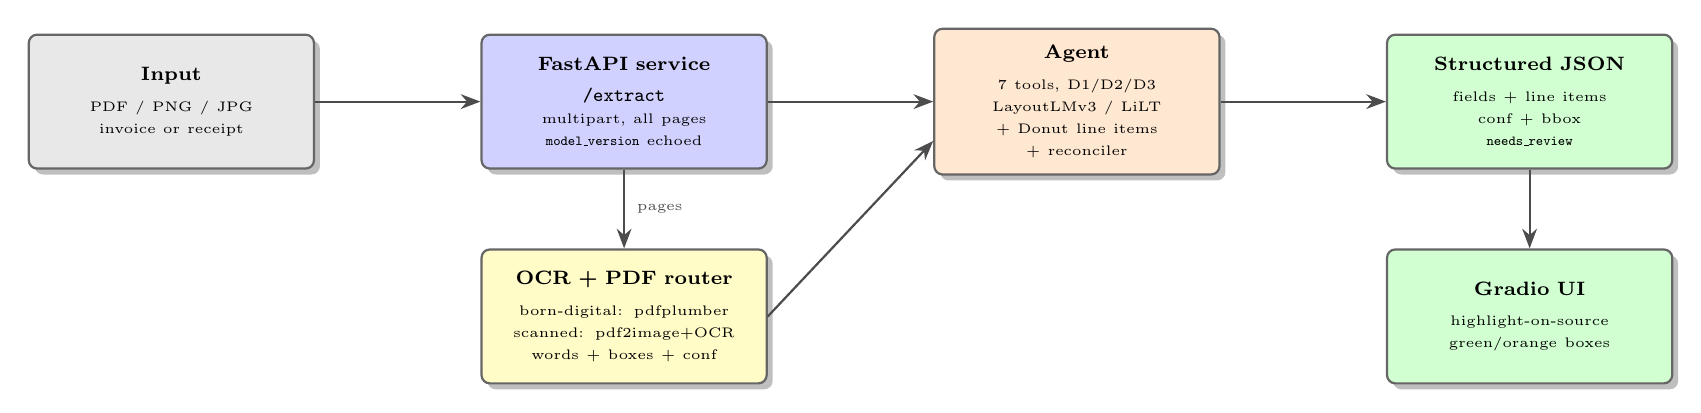
\begin{tikzpicture}[
  node distance=1.0cm and 2.1cm,
  box/.style={rectangle, draw=black!60, rounded corners=3pt, thick,
             text width=3.2cm, minimum height=1.7cm, align=center,
             inner sep=6pt, font=\scriptsize, drop shadow},
  inbox/.style={box, fill=gray!18},
  ocrbox/.style={box, fill=yellow!22},
  modelbox/.style={box, fill=orange!18},
  apibox/.style={box, fill=blue!18},
  uibox/.style={box, fill=green!18},
  arrow/.style={-{Stealth[length=2.5mm]}, thick, color=black!70}
]

\node[inbox] (doc) {%
  \textbf{Input}\\[3pt]
  {\tiny PDF / PNG / JPG}\\
  {\tiny invoice or receipt}
};
\node[apibox, right=of doc] (api) {%
  \textbf{FastAPI service}\\[3pt]
  \texttt{/extract}\\
  {\tiny multipart, all pages}\\
  {\tiny \texttt{model\_version} echoed}
};
\node[ocrbox, below=1.0cm of api] (ocr) {%
  \textbf{OCR + PDF router}\\[3pt]
  {\tiny born-digital: pdfplumber}\\
  {\tiny scanned: pdf2image+OCR}\\
  {\tiny words + boxes + conf}
};
\node[modelbox, right=of api] (agent) {%
  \textbf{Agent}\\[3pt]
  {\tiny 7 tools, D1/D2/D3}\\
  {\tiny LayoutLMv3 / LiLT}\\
  {\tiny + Donut line items}\\
  {\tiny + reconciler}
};
\node[uibox, right=of agent] (out) {%
  \textbf{Structured JSON}\\[3pt]
  {\tiny fields + line items}\\
  {\tiny conf + bbox}\\
  {\tiny \texttt{needs\_review}}
};
\node[uibox, below=1.0cm of out] (ui) {%
  \textbf{Gradio UI}\\[3pt]
  {\tiny highlight-on-source}\\
  {\tiny green/orange boxes}
};

\draw[arrow] (doc) -- (api);
\draw[arrow] (api) -- node[right=1pt, font=\tiny] {pages} (ocr);
\draw[arrow] (ocr.east) -- ([yshift=-5mm]agent.west);
\draw[arrow] (api) -- (agent);
\draw[arrow] (agent) -- (out);
\draw[arrow] (out) -- (ui);

\end{tikzpicture}%
}
\caption{Deployment architecture. The FastAPI service ingests a document, routes PDFs (born-digital vs scanned) through OCR, and hands words+boxes to the agent (LayoutLMv3/LiLT + Donut + reconciler) which returns structured JSON with per-field confidence, bounding boxes, and a \texttt{needs\_review} flag. The Gradio UI renders the result as a highlight-on-source view. The optional LLM-vision fallback is feature-flagged and isolated.}
\label{fig:arch}
\end{figure}

\subsection{The \texttt{POST /extract} Contract}

\texttt{POST /extract} accepts \texttt{multipart/form-data} (\texttt{file}: png/jpg/pdf,
optional \texttt{doc\_type}, \texttt{return\_crops}, \texttt{min\_confidence} default
0.80) and returns normalized, per-page-merged JSON:

\begin{lstlisting}[basicstyle=\ttfamily\footnotesize]
{
  "request_id": "req_7f3a9c",
  "model_version": "layoutlmv3-kie-2026-06-20-a1b2c3d",
  "doc_type": "invoice", "page_count": 2, "processing_ms": 312,
  "fields": {
    "vendor":     {"value":"Acme Corp Ltd","confidence":0.97,"bbox":[62,40,310,72],"page":1},
    "date":       {"value":"2026-05-14","confidence":0.93,"bbox":[420,40,560,70],"page":1,"raw":"14/05/2026"},
    "invoice_no": {"value":"INV-2026-00871","confidence":0.95,"bbox":[420,80,560,108],"page":1},
    "currency":   {"value":"USD","confidence":0.88,"bbox":[500,640,540,668],"page":1},
    "subtotal":   {"value":1240.00,"confidence":0.91,"page":1},
    "tax":        {"value":124.00,"confidence":0.90,"page":1},
    "total":      {"value":1364.00,"confidence":0.96,"page":1}
  },
  "line_items": [ {"desc":{"value":"Widget A","confidence":0.92},
     "qty":{"value":10,"confidence":0.94}, "unit_price":{"value":24.00,"confidence":0.89},
     "amount":{"value":240.00,"confidence":0.90}, "page":1, "row":0} ],
  "confidence": 0.92, "needs_review": false, "review_reasons": [],
  "warnings": ["currency inferred from symbol"],
  "coordinate_space": {"system":"pixel_topleft","page_dims":[[612,792],[612,792]]}
}
\end{lstlisting}

\noindent\textbf{\texttt{needs\_review} triggers} (any one sets it \texttt{true}): a
required field (\texttt{total}, \texttt{date}, \texttt{vendor}, \texttt{invoice\_no})
below \texttt{min\_confidence}; \textbf{arithmetic fails}
($|\text{subtotal}+\text{tax}-\text{total}| > 0.02\cdot\text{total}$ or
$\sum$\,line amounts $\neq$ subtotal); doc-type confidence $<0.70$; or no total / too few
OCR tokens. Bounding boxes are returned in \textbf{pixel coordinates, top-left origin},
per source page (the model's 0--1000 boxes de-normalized for the UI). The error envelope
uses codes \texttt{400}, \texttt{413 FILE\_TOO\_LARGE} (cap $\approx$20\,MB / 15 pages),
\texttt{415}, \texttt{422 NO\_TEXT\_DETECTED}, \texttt{429}, \texttt{500}, and
\texttt{503 MODEL\_LOADING}.

\subsection{Latency Targets and Batching}

\begin{table}[H]
\centering
\caption{Latency budget (per-stage and end-to-end)}
\begin{tabular}{lcc}
\toprule
\textbf{Path} & \textbf{GPU (H100/A10)} & \textbf{CPU (8 vCPU)} \\
\midrule
OCR (Tesseract, 1 page)                 & 150--400\,ms  & 150--400\,ms \\
LayoutLMv3 KIE forward (1 page, $\leq$512 tok) & 15--40\,ms & 200--600\,ms \\
Donut forward (generate, 1 page)        & 300--800\,ms  & 4--10\,s (avoid) \\
\textbf{End-to-end \texttt{/extract}, 1-page image} & \textbf{$\approx$250--500\,ms p95} & \textbf{$\approx$0.8--1.5\,s p95} \\
\bottomrule
\end{tabular}
\end{table}

\textbf{Dynamic batching}: queue inference and flush on \texttt{max\_batch=16} or
\texttt{max\_wait=20ms}; OCR (the bottleneck) runs in a CPU process pool while the GPU
forward is a batched micro-service; models are kept warm and \texttt{/health} returns
\texttt{503 MODEL\_LOADING} until weights are resident.

\subsection{Model Versioning}

Every artifact is tagged \texttt{\{family\}-\{date\}-\{git\_sha\}} (e.g.
\texttt{layoutlmv3-kie-2026-06-20-a1b2c3d}) and echoed in every response
(\texttt{model\_version}) and in \texttt{/metrics}. The registry resolves a semantic
alias (\texttt{@prod}, \texttt{@canary}) to a pinned revision sha at boot; the
\texttt{label\_map} / \texttt{id2label} / processor config are stored alongside the
weights, and \texttt{transformers} / OCR-engine versions are pinned and recorded in
\texttt{/health}.

% ============================================================
\section{Agentic AI Component}
% ============================================================

\subsection{Agent Architecture}

The agent is \textbf{not} an LLM prompt loop. It is a deterministic \textbf{state
machine} whose policy is a rules engine, operating over a single shared
\texttt{AgentState} \emph{blackboard} so the entire run is reproducible and auditable via
a step \texttt{trace}. Seven \texttt{state\,$\to$\,state} tools mutate and return the
blackboard; none requires a paid API except the isolated, optional
\texttt{llm\_vision\_fallback}.

\begin{enumerate}\setlength\itemsep{0.15em}
  \item \textbf{\texttt{classify\_document}} (\textit{tool}): doc-type (invoice/receipt/other) + scan-quality (Laplacian-variance blur + skew + DPI).
  \item \textbf{\texttt{run\_ocr}} (\textit{tool}): words + per-token confidence + boxes; native PDF text layer if digital, else Tesseract/PaddleOCR. \emph{Re-runnable with a different engine on retry.}
  \item \textbf{\texttt{extract\_layout}} (\textit{tool}): header fields via fine-tuned LayoutLMv3/LiLT (confidence = mean softmax over the field's tokens).
  \item \textbf{\texttt{extract\_line\_items}} (\textit{tool}): table rows via bbox row/col clustering --- \texttt{qty} and \texttt{unit\_price} make per-line math checkable (the reference lacked this).
  \item \textbf{\texttt{validate}} (\textit{decision-making}): the heart of the agent --- pure rules, arithmetic reconciliation (see below).
  \item \textbf{\texttt{normalize}} (\textit{tool}): ISO-8601 dates, \texttt{Decimal(str(x))} 2-dp money, ISO-4217 currency.
  \item \textbf{\texttt{llm\_vision\_fallback}} (\textit{optional tool}): the reference's GPT-4o-vision call, demoted to a feature-flagged fallback. No API key $\Rightarrow$ unavailable $\Rightarrow$ agent proceeds to human review. The system stays fully functional offline.
\end{enumerate}

\paragraph{\texttt{validate} checks.} \texttt{reconcile}:
$\sum(\text{item.amount}) = \text{subtotal}\,(\pm\varepsilon)$,
$\text{subtotal}+\text{tax} = \text{total}\,(\pm\varepsilon)$, and
$\text{tax}\approx\text{subtotal}\cdot\text{tax\_rate}$ if present;
\texttt{per\_line}: $\text{qty}\cdot\text{unit\_price}=\text{amount}\,(\pm\varepsilon)$;
\texttt{date\_valid}, \texttt{invoice\_no} plausible, \texttt{currency} detected,
\texttt{required\_present} (\texttt{invoice\_number}, \texttt{invoice\_date},
\texttt{total}, \texttt{issuer}); and tolerance
$\varepsilon = \max(0.01,\,0.005\cdot\text{total})$ so penny rounding is tolerated but
real gaps are not.

\subsection{The Three Decision Points}

\begin{table}[H]
\centering
\caption{The three explicit decision points (config-tunable thresholds)}
\small
\begin{tabularx}{\linewidth}{@{} c l L @{}}
\toprule
\textbf{\#} & \textbf{Where} & \textbf{Condition $\to$ Action} \\
\midrule
\textbf{D1} & after \texttt{classify\_document} & \texttt{doc\_type == OTHER} $\to$ stop / route out. \newline \texttt{scan\_quality $<$ Q\_MIN} or \texttt{ocr\_mean\_conf $<$ OCR\_MIN} $\to$ retry (rescan / switch OCR engine / deskew); after \texttt{MAX\_OCR\_ATTEMPTS} $\to$ \textbf{HUMAN REVIEW}. \\
\addlinespace
\textbf{D2} & after \texttt{validate} & \texttt{not reconciles} \textbf{OR} \texttt{missing\_required} \textbf{OR} any required field \texttt{conf $<$ FIELD\_CONF\_MIN} $\to$ if LLM fallback available \& untried, escalate \& re-validate; else $\to$ \textbf{HUMAN REVIEW} with reasons. \\
\addlinespace
\textbf{D3} & final gate & \texttt{reconciles AND no missing\_required AND overall\_confidence $\geq$ AUTO\_MIN} $\to$ \textbf{AUTO-APPROVE}; otherwise $\to$ \textbf{HUMAN REVIEW} (attach reasons + bboxes). \\
\bottomrule
\end{tabularx}
\end{table}

\noindent\textbf{Thresholds:} $Q_{\min}=0.45$, $\text{OCR}_{\min}=0.70$,
$\text{FIELD\_CONF}_{\min}=0.80$, $\text{AUTO}_{\min}=0.85$,
$\text{MAX\_OCR\_ATTEMPTS}=2$, $\varepsilon=\max(0.01,0.005\cdot\text{total})$. The
\textbf{conservative confidence bottleneck}
$\text{overall\_confidence} = \min(\text{doc\_type\_conf},\,\text{ocr\_mean\_conf},\,\min(\text{required-field confidences}))$
ensures one shaky required field blocks auto-approval.

\begin{figure}[H]
\centering
\resizebox{\linewidth}{!}{%
\begin{tikzpicture}[
  node distance=0.30cm,
  step/.style={rectangle, draw=black!60, rounded corners=2pt, thick,
              text width=13.5cm, inner sep=5pt, minimum height=0.7cm,
              align=center, font=\footnotesize},
  inn/.style={step, fill=gray!15},
  tool/.style={step, fill=blue!13},
  model/.style={step, fill=purple!13},
  dec/.style={step, fill=red!12},
  approve/.style={step, fill=green!18},
  review/.style={step, fill=yellow!22},
  arrow/.style={-{Stealth[length=2mm]}, thick}
]

\node[inn] (s0) {\textbf{Ingest} PDF/PNG/JPG --- load \emph{all} pages into \texttt{AgentState}};
\node[tool, below=of s0] (s1) {\textbf{1. \texttt{classify\_document}} $\to$ doc\_type + scan\_quality \quad\textbf{[D1]}};
\node[tool, below=of s1] (s2) {\textbf{2. \texttt{run\_ocr}} $\to$ words + boxes + conf \quad\textbf{[D1 gate]} retry / switch engine / deskew (\texttt{MAX\_OCR\_ATTEMPTS}); else \textbf{REVIEW}};
\node[model, below=of s2] (s3) {\textbf{3. \texttt{extract\_layout}} (LayoutLMv3/LiLT) $+$ \textbf{4. \texttt{extract\_line\_items}} (Donut / clustering)};
\node[tool, below=of s3] (s4) {\textbf{6. \texttt{normalize}} (ISO dates, Decimal money, ISO-4217) $\to$ \textbf{5. \texttt{validate}} (reconcile + per-line + checks)};
\node[dec, below=of s4] (s5) {\textbf{[D2]} not reconciles \textbf{OR} missing\_required \textbf{OR} low conf? \quad if so $\to$ \textbf{7. \texttt{llm\_vision\_fallback}} (optional) $\to$ re-validate; else $\to$ \textbf{REVIEW}};
\node[dec, below=of s5] (s6) {\textbf{[D3]} reconciles \textbf{AND} complete \textbf{AND} overall\_confidence $\geq$ AUTO\_MIN?};
\node[approve, below left=0.5cm and -3cm of s6] (ap) {\textbf{AUTO-APPROVE} $\to$ post to ledger};
\node[review, below right=0.5cm and -3cm of s6] (rv) {\textbf{HUMAN REVIEW} $\to$ queue (reasons + bboxes)};

\foreach \a/\b in {s0/s1, s1/s2, s2/s3, s3/s4, s4/s5, s5/s6}
  \draw[arrow] (\a) -- (\b);
\draw[arrow] (s6) -- node[left=1pt, font=\tiny] {yes} (ap);
\draw[arrow] (s6) -- node[right=1pt, font=\tiny] {no} (rv);

\end{tikzpicture}%
}
\caption{The agent pipeline: seven \texttt{state\,$\to$\,state} tools over a shared blackboard with three decision points (D1 doc-type/quality + OCR retry; D2 validation with optional LLM escalation; D3 final confidence gate). The arithmetic reconciler in step 5 is the core safety mechanism the reference lacks.}
\label{fig:agent}
\end{figure}

\subsection{Worked Example --- Totals Don't Reconcile $\to$ Flagged}

\textbf{Input:} \texttt{INV-2024-077.pdf}, a clean digital-PDF invoice. Two lines:
\emph{Consulting services} ($10\times150.00=1{,}500.00$) and \emph{Onboarding setup}
($1\times300.00=300.00$). Header: \texttt{subtotal=1,800.00}, \texttt{tax\_rate=20\%},
\texttt{tax=360.00}, \textbf{\texttt{total=1,860.00}} (the printed total is itself wrong),
\texttt{currency=GBP}, all field confidences $\geq 0.90$.

\begin{lstlisting}[basicstyle=\ttfamily\footnotesize]
# Agent trace
1) classify_document -> INVOICE, conf 0.97, scan_quality 0.92         (D1: pass)
2) run_ocr           -> engine=native_pdf, ocr_mean_conf=0.99         (D1 gate: pass)
3) extract_layout + extract_line_items -> 7 fields + 2 line items
4) normalize         -> date already ISO; amounts -> Decimal; currency -> GBP
5) validate:
     per-line:  10x150.00=1,500.00 OK ; 1x300.00=300.00 OK
     sum(lines)=1,800.00 == subtotal 1,800.00 OK
     tax: 1,800.00 x 20% = 360.00 == tax 360.00 OK
     RECONCILE total: expected subtotal+tax = 2,160.00 ; printed total = 1,860.00
       reconcile_delta = -300.00 ;  e = max(0.01, 0.005*1,860) = 9.30
       |-300.00| > 9.30  ->  reconciles = False
6) D2: needs_help=True. LLM fallback (if enabled) re-reads the same printed 1,860.00
       (document is genuinely inconsistent) -> re-validation still fails.
7) D3: reconciles == False  ->  NOT auto-approved
8) finish(NEEDS_REVIEW), review_reasons=
     ["totals don't reconcile: total=1860.00 vs subtotal+tax=2160.00 (off by -300.00)"]
   Review payload carries every field's bbox -> UI highlights the printed total
   and both line items for a 5-second human confirmation.
\end{lstlisting}

\textbf{Contrast with the reference.} \texttt{ruizguille}'s pipeline would
\texttt{Invoice(**data)} successfully (1,860.00 is a valid float), write
\texttt{Total=1860.00} into Excel, and \emph{silently} add \pounds1,860 to revenue and
\pounds360 to the tax summary --- the \pounds300 discrepancy vanishes into the
aggregates. Our agent \textbf{catches it and routes to a human}. That single arithmetic
check --- combined with Decimal money, multi-page handling, per-field confidence, and
offline operation --- is the core value-add and the basis for the strict-dominance
claim.

% ============================================================
\section{Continual Learning \& Monitoring}
% ============================================================

\subsection{The Corrections Flywheel}

Every uncertain document a human touches becomes future training signal. Two streams
feed the retraining corpus, both already emitted by the running pipeline:
\begin{itemize}\setlength\itemsep{0.15em}
  \item \textbf{Human corrections} (\textit{gold}): \texttt{POST /review-queue/\{id\}} stores \texttt{corrected\_fields} + \texttt{verdict}, keyed to \texttt{request\_id} and \texttt{model\_version}, with \texttt{stored\_for\_retraining=true}.
  \item \textbf{Extraction logs} (\textit{silver}): every \texttt{/extract} call logs the full \texttt{AgentState.trace} (OCR tokens+boxes, per-field \texttt{FieldValue}, \texttt{ValidationReport}, \texttt{review\_reasons}).
\end{itemize}
Because LayoutLMv3/LiLT predictions are grounded to OCR tokens with bboxes, a correction
maps straight back to \texttt{words + boxes + label} --- a directly re-trainable example
in the canonical schema. Every flagged document is, by construction, a hard negative:
this is the closed loop the reference cannot have (it has no confidence, no queue, no
corrections).

\subsection{Retraining: Champion / Challenger + Canary}

On a fixed cadence (or when $\geq N$ new corrections accumulate), the autopilot
continue-trains a \textbf{challenger} from the current champion checkpoint, on
corrections \emph{mixed with the original splits} to avoid catastrophic forgetting. The
challenger must match or beat the champion on a \textbf{frozen evaluation set}
(per-entity seqeval F1 --- a challenger that lifts overall F1 but collapses
\texttt{TOTAL} is rejected). It is then canaried on a small slice of \texttt{/extract}
traffic; promotion requires the \textbf{needs-review rate not to rise} and field-F1 to
hold or improve, otherwise the registry alias auto-rolls back to the previous pinned sha.

\subsection{Monitoring \& Degradation Detection}

The monitoring module exposes Prometheus metrics at \texttt{GET /metrics}:
\texttt{field\_confidence\{field,quantile\}}, \texttt{extract\_needs\_review\_total}
(by \texttt{review\_reasons}), \texttt{extract\_latency\_seconds\_bucket} (per-stage,
GPU vs CPU), validation pass-rate, and \texttt{extract\_requests\_total}. Three
independent signals must all be defeated for a regression to hide:
\begin{itemize}\setlength\itemsep{0.15em}
  \item \textbf{Frozen-eval F1} --- per-entity F1 on a version-pinned eval set re-scored each release; the absolute yardstick separating ``model got worse'' from ``inputs got harder''.
  \item \textbf{Needs-review-rate spike} --- a rising rate with \emph{clean} OCR but low field confidence indicates new vendor templates (input drift) $\to$ curate + retrain, not roll back.
  \item \textbf{OCR-confidence drift} --- the \texttt{ocr\_mean\_conf} distribution sinking below \texttt{OCR\_MIN} more often.
\end{itemize}
The design guarantee: a drift the model cannot yet handle never produces a silent wrong
answer --- it fails the validator or the confidence gate and lands in the review queue,
\emph{which is exactly where the next batch of training data comes from}.

% ============================================================
\section{Data Privacy \& Model Robustness}
% ============================================================

\subsection{Privacy}

\begin{itemize}\setlength\itemsep{0.15em}
  \item \textbf{Offline-first by design}: the default path needs no network, so invoices (vendor, customer, and tax identifiers) stay on-premises.
  \item \textbf{PII handling}: invoices carry sensitive identifiers; retention rules apply to the review queue, and a legal sign-off gate guards any non-commercially-licensed asset.
  \item \textbf{No mandatory cloud}: the only cloud tool (\texttt{llm\_vision\_fallback}) is feature-flagged; with no API key, the system runs fully offline.
  \item \textbf{Secrets via environment variables}; no hard-coded credentials.
\end{itemize}

\subsection{Robustness}

\begin{itemize}\setlength\itemsep{0.15em}
  \item \textbf{OCR quality}: multi-engine retry (native-PDF $\to$ PaddleOCR $\to$ docTR), deskew/denoise/upscale on retry, gated by \texttt{OCR\_MIN=0.70} after \texttt{MAX\_OCR\_ATTEMPTS}.
  \item \textbf{Bbox/label-alignment bugs} (the \#1 silent accuracy killer): enforce 0--1000 normalization, unit-test that continuation subwords/special tokens become \texttt{-100}, assert \texttt{len(words)==len(boxes)==len(labels)}.
  \item \textbf{Multi-page PDFs}: process \emph{all} pages (the reference loses all but page 1); retain a \texttt{page} index in every bbox; merge headers, concatenate line items, reconcile totals across pages.
  \item \textbf{Float-money errors}: \texttt{Decimal(str(x))} 2-dp and ISO-4217 currency detection, reconciled with $\varepsilon=\max(0.01,0.005\cdot\text{total})$ so pennies are tolerated without masking real gaps.
  \item \textbf{Graceful degradation}: an LLM-fallback outage is a \emph{quality} event (more human review), not an availability incident.
\end{itemize}

% ============================================================
\section{Project Management}
% ============================================================

This project was completed \textit{individually}; the five roles below are
\textbf{simulated} to model how the work would be split in a real team. The critical
path is \textbf{Data\,+\,OCR $\to$ LayoutLMv3 training $\to$ validation agent}, because
the agent's value (arithmetic reconciliation) depends on trustworthy fields, which
depend on correctly bbox-normalized training data.

\begin{table}[H]
\centering
\caption{Project timeline (7 weeks, with exit gates)}
\small
\begin{tabularx}{\linewidth}{@{} c l L @{}}
\toprule
\textbf{Wk} & \textbf{Phase} & \textbf{Deliverable / exit gate} \\
\midrule
1 & Scope \& scaffold     & \texttt{invoice\_ai} package + configs (thresholds) + canonical schema reviewed \\
2 & Data + OCR pipeline   & loaders + PDF router + OCR (words/boxes/conf); boxes normalized 0--1000 \\
3 & LayoutLMv3 training   & fine-tuned LayoutLMv3 \& LiLT; per-entity F1 reported (no hidden collapse) \\
4 & Line-items + agent    & Donut path + \texttt{AgentState} + reconciler + D1/D2/D3; \texttt{INV-2024-077} routes to review \\
5 & API + UI              & FastAPI endpoints + Gradio highlight demo + Docker; p95 within budget \\
6 & Evaluation            & seqeval F1, field accuracy, line-item F1, pass-rate, latency GPU vs CPU \\
7 & Docs / report         & report + slides + reproducible notebook; ids/metrics match the brief \\
\bottomrule
\end{tabularx}
\end{table}

\textbf{Scaling reflection.} A real team would invest in the operational layers a solo
build can only stub: an annotation UI reusing the same highlight-on-source view; active
learning from the review queue (prioritizing reconciliation failures); GPU inference ops
(dynamic batching, OCR in a CPU pool, canary rollout); on-call alerting on the Prometheus
signals; and a data-governance gate enforcing the license posture (LayoutLMv3 internal
only; LiLT/Donut commercial).

% ============================================================
\section{Ethics \& Responsible AI}
% ============================================================

\subsection{Who Benefits}

Finance and accounting teams (faster, auditable extraction), auditors (bbox provenance
for fast confirmation), and organizations (fewer silent ledger errors, on-premises
privacy).

\subsection{Who Could Be Harmed}

Over-reliance on automation could let a wrong field slip through if the human reviewer
rubber-stamps the queue; vendors could be mis-attributed if OCR/extraction errors are
not caught. The design mitigates both: the conservative confidence bottleneck surfaces
genuinely shaky fields, and \textbf{nothing is auto-posted unless the arithmetic
reconciles}.

\subsection{The Core Responsible-AI Mechanism}

The validation reconciler is the ethical centerpiece: the system \textbf{never silently
accepts a total that does not add up}. Where the reference would coerce a wrong float and
post it to the ledger, this agent flags it for a human with the exact source box. This
turns the model from an unaccountable oracle into an \emph{accountable, auditable}
assistant.

\subsection{Misuse Risks and License Posture}

\begin{itemize}\setlength\itemsep{0.15em}
  \item \textbf{License}: LayoutLMv3 is CC-BY-NC-SA-4.0 (non-commercial) --- using it in a paid deployment would be a license violation; the commercial path ships LiLT/Donut (MIT). This is a governance decision, not a footnote.
  \item \textbf{Data}: SROIE/FUNSD are research-challenge data; commercial use requires legal sign-off.
  \item \textbf{Automation bias}: human review must be a genuine check, not a rubber stamp; the bbox highlight UI makes a real 5-second confirmation feasible.
\end{itemize}

% ============================================================
\newpage
\begin{thebibliography}{9}

\bibitem{layoutlmv3} Huang, Y., Lv, T., Cui, L., Lu, Y., \& Wei, F. (2022). LayoutLMv3: Pre-training for Document AI with Unified Text and Image Masking. \textit{ACM MM 2022}.

\bibitem{lilt} Wang, J., Jin, L., \& Ding, K. (2022). LiLT: A Simple yet Effective Language-Independent Layout Transformer for Structured Document Understanding. \textit{ACL 2022}.

\bibitem{donut} Kim, G., et al. (2022). OCR-free Document Understanding Transformer (Donut). \textit{ECCV 2022}.

\bibitem{sroie} Huang, Z., et al. (2019). ICDAR 2019 Competition on Scanned Receipt OCR and Information Extraction (SROIE).

\bibitem{cord} Park, S., et al. (2019). CORD: A Consolidated Receipt Dataset for Post-OCR Parsing. \textit{NeurIPS 2019 Workshop on Document Intelligence}.

\bibitem{funsd} Jaume, G., Ekenel, H.\,K., \& Thiran, J.-P. (2019). FUNSD: A Dataset for Form Understanding in Noisy Scanned Documents. \textit{ICDAR-OST 2019}.

\bibitem{huggingface} Wolf, T., et al. (2020). Transformers: State-of-the-Art Natural Language Processing. \textit{EMNLP 2020}.

\bibitem{seqeval} Nakayama, H. (2018). seqeval: A Python framework for sequence labeling evaluation. \url{https://github.com/chakki-works/seqeval}

\bibitem{fastapi} Ram\'irez, S. (2018). FastAPI. \url{https://fastapi.tiangolo.com/}

\bibitem{paddleocr} Du, Y., et al. (2020). PP-OCR: A Practical Ultra Lightweight OCR System. \url{https://github.com/PaddlePaddle/PaddleOCR}

\bibitem{reference} Guillermo Ruiz. \textit{invoice-processing} (reference implementation, MIT). \url{https://github.com/ruizguille/invoice-processing}

\end{thebibliography}

\end{document}
